	We start the stability analysis for the linear case since the 
stability conditions
for the solution of the linear SDE in both additive and multiplicative cases are well
known. So,  we first recall these conditions for the continuous case and later obtain
sufficient conditions to ensure stability  and asymptotic stability in mean and mean
square for the explicit Steklov method \eqref{Steklov}. Moreover in the additive case,
we analyze the stability in a path-wise sense based on the work of Buckwar et al.
\cite{Buckwar2011a}.
\subsection{Multiplicative noise}
		For the linear multiplicative SDE \eqref{SDE},  its zero equilibrium solution is
	called {\it mean stable} if $\lim_{t\to\infty}\m y(t)=0$, and it is said to be {\it
	mean square stable} if  $\lim_{t\to\infty}\ms{y(t)}=0$. Then the zero solution of
	\eqref{SDE} is mean stable if $\lambda<0$ and it is    mean square stable if
	$Re(\lambda)+\frac{1}{2} |\xi|^2 <0$, see \cite{Higham2000}. In order to obtain the
	explicit Steklov approximation \eqref{Steklov} for equation \eqref{SDE}, we use the
	function $\Psi_h$  defined in \eqref{psi1} so the linear Steklov discretization is
	written as follows:
	\begin{equation}\label{eqn:SteklovMN}
		Y_{n+1}=\exp(\lambda h)Y_n+\xi Y_n \Delta W_n.
	\end{equation}
	Similarly, we say that the method \eqref{eqn:SteklovMN} is {\it mean stable} if
	$\lim_{n\to\infty} \m Y_n=0$, and we called it {\it mean square stable} if
	$\lim_{n\to\infty}\ms{Y_{n}}=0$. Moreover, a stochastic numerical method is    {\it
	$\mathcal{A}$-stable} in some sense, if it is stable for all step size $h$ when its
	associated continuous SDE is stable in the same sense.
	\begin{pro}
		Let $\lambda<0$, then the explicit Steklov method \eqref{eqn:SteklovMN} for the
		SDE \eqref{SDE} is  $\mathcal{A}$-stable in mean. Moreover, it is mean square
		stable if 
		\begin{equation}\label{c2}
			\exp \lftrght{2Re(\lambda h)}{(}{)}
			+|\xi|^2 h<1.
	\end{equation}
	\end{pro}
	\begin{proof}
		Denoting by  $p=\exp(\lambda h)$ and  $q=\xi\sqrt{h}$, we can  rewrite the Steklov
		method \eqref{eqn:SteklovMN}  as
		\begin{equation}\label{eq2}
			Y_{n+1}=(p+qV_n)Y_n.
		\end{equation}
		Taking expectation in \eqref{eq2} and iterating this recurrence  until the initial
		step, we obtain
		\begin{equation}\label{eq3}
			\m{Y_n}=(p)^{n+1}\m{Y_0},
		\end{equation}
		thus the limit of the sequence \eqref{eq3} as $n$ approaches infinity is zero for
		$\lambda<0$. Now, applying square modulus to \eqref{eq2}  and carrying out an
		analogous procedure, it follows that:
		\begin{eqnarray*}
			\ms{Y_n^h}
			&=&(|p|^2+|q|^2)^{n+1}\ms{Y_0^h}.
		\end{eqnarray*}
		Therefore the sequence $\ms{Y_n^h}$ approaches to zero as $n$ tends to infinity if
		and only if  $|p|^2+|q|^2<1$.
	\end{proof}
			In \Cref{fig:1}, we show a comparison between the mean square stability region of
	the zero solution for the linear SDE and the associated explicit Steklov and
	Euler-Maruyama approximations  \cite{Higham2000b}.
	\begin{figure}[h!]
			\begin{center}
				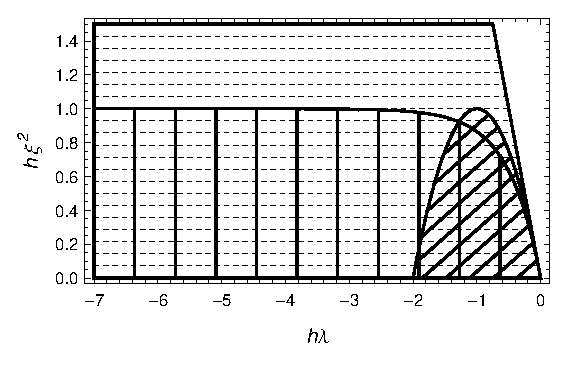
\includegraphics{./papers/paperA/figures/StabilityPlotMultiplicativeNoise.eps}
				%\import{figures/}{StabilityPlotMultiplicativeNoise.eps}
			\end{center}
		\caption{
			Mean square stability regions: horizontal lines represent the region for the linear
			SDE \eqref{SDE}, the vertical lines form the explicit Steklov region and the
			diagonal lines draw the Euler-Maruyama region.
		}%
			\label{fig:1}
		\end{figure}
		\subsection{Additive noise}
		Here we study the additive linear SDE: 
		\begin{equation}\label{SDEa}
			dy(t)=\lambda y(t)dt+ \xi  dW(t) , \qquad X_{t_0}=x_{t_0}.		
		\end{equation}
		where $\lambda$, $\xi \in \mathbb{C}$ and $X_{t_0}$ is the initial value of the process
		at time $t_0$. Equation \eqref{SDEa}  has  the following  exact solution:
	\begin{equation}\label{eqn:OUProcess}
		y(t)=\exp(\lambda (t-t_0)) y(t_0)+\xi 
		\exp(\lambda t)\int\limits_{t_0}^{t}\exp(-\lambda s)dW(s), 
		\qquad t\geq t_0.
	\end{equation}
	The stochastic process $y(t)$ defined in \eqref{eqn:OUProcess} is known as 
	the {\it Ornstein-Uhlenbeck}'s (OU)  process. According to \cite{Hernandez1992},
	the OU process  is {\it asymptotically mean stable} if
		$ \lim_{t\to\infty}\m{y(t)}=0$ and is
	{\it  asymptotically  mean square stable} if
	$\displaystyle \lim_{t\to\infty}\ms{y(t)}=-\xi/2Re(\lambda)$. Both 
	limits are verified if $\lambda<0$. Now, the explicit 
	Steklov recurrence  to solve additive linear SDE is
	\begin{equation}\label{eqn:LinearSteklovRecurrence}
		Y_{n+1} =\exp(\lambda h)Y_n+\xi \Delta W_n.
	\end{equation}
	Analogous stability properties are given for 
	stochastic  difference equations with additive noise \cite{SaiotoPreprint}. 
	Next, we  prove {\it mean-square consistency} for the explicit Steklov, 
	that is, $$\lim_{h\to 0}\Big(\lim_{n\to\infty} \ms{Y_n}\Big)=-\xi/2Re(\lambda).$$ 
%
	\begin{pro}
		Let $\lambda<0$, the explicit Steklov method  
		\eqref{eqn:LinearSteklovRecurrence} for the additive linear SDE \eqref{SDEa}
		is  $\mathcal{A}$-stable in mean and  mean-square consistent.	
	\end{pro}
	\begin{proof}  
		Taking the expected value of \eqref{eqn:LinearSteklovRecurrence} and iterating
		backwards this recurrence we obtain the identity \eqref{eq3}, so the
		$\mathcal{A}$-stability in mean is verified for $\lambda<0$. Now, taking the mean
		square of the recurrence \eqref{eqn:LinearSteklovRecurrence} and after some algebraic
		manipulations we get
		\begin{eqnarray*}\label{eqn:SteklovMS-Stable1}
			\ms{Y_{n+1}}&
			=&\exp(2Re(\lambda)h)
				\ms{Y_n}+|\xi|^2 h\\
			&=& 
				\ms{Y_{0}}+|\xi|^2h
				\{1+\cdots+
				\exp(2n Re(\lambda) h)\}
				\ms{Y_{n+1}}\\
			&=&
				\exp(2n Re(\lambda) h)
				\ms{Y_0}
				+\xi^2 h
				\frac{[\exp(2Re(\lambda)h)]^{n+1}-1}{\exp(2Re(\lambda)h)-1}.
		\end{eqnarray*}
		Given that $\lambda<0$
		\begin{eqnarray*}
		\lim_{\substack{ n\to \infty\\ h\to 0}}
		\ms{Y_{n+1}}=\lim_{\substack{ n\to \infty\\ h\to 0}}
		\frac{-|\xi|^2 h}{\exp(2Re(\lambda)h)-1}=
		-\frac{|\xi|^2}{2Re(\lambda)}.
		\end{eqnarray*}
	\end{proof}
	So far we have analyzed  the asymptotic behavior of the forward motion for the explicit
	Steklov method  \eqref{eqn:LinearSteklovRecurrence}. Now, if we consider $\lambda<0$
	then the OU solution \eqref{eqn:OUProcess} does not convergence as $t$ tends to infinity
	but has the following pullback limit:
	\begin{equation}\label{eq4}
		\lim_{t_0\to-\infty} y(t)=\widehat{O}_t:=
		\exp(\lambda t)\int\limits_{-\infty}^{t}\exp(-\lambda s)dW(s), 
	\end{equation}
	$B_t$  is now defined for all $t\in\mathbb{R}$, see
	\cite{Arnold1998, kloeden1999towards}. Furthermore, the process \eqref{eq4} is a
	stationary solution  of the additive linear SDE which attracts all other solutions in
	forward time and path-wise sense. Moreover, it is a finite process for all $t\geq
	T_{D(\omega)}$ ($\omega\in \Omega$) for  appropriate families $D(\omega)$ of bounded
	sets of initial conditions, see \cite{Robinson2002}. Therefore, a study of the pullback
	asymptotic behavior for the Steklov stochastic method
	\eqref{eqn:LinearSteklovRecurrence} is important in the additive case and in the next
	subsection we carry it out based on Caraballo and Kloeden's work  \cite{Caraballo2006}.
	\subsubsection{Path-wise linear stability}
		Here we obtain a stationary discrete process $\widehat{O}_n^{(h)}$ for the linear explicit
		Steklov  and  prove that converges to the continuous process \eqref{eq4}. 
	\begin{pro}
		Let $\lambda<0$, the explicit Steklov method \eqref{eqn:LinearSteklovRecurrence} for
		the additive linear SDE \eqref{SDEa} has the following attractor: 
		\begin{equation}\label{O}
			\widehat{O}_n^{(h)}  :=
			\xi \sum_{j=-\infty}^{n-1}\exp(\lambda h(n-1-j)) \Delta W_j,
		\end{equation}
		for any positive step size $h$. Moreover, it converges to the Ornstein-Uhlenbeck's
		process \eqref{eq4}.
	\end{pro}
	\begin{proof}
		We consider a recurrence given  by the Steklov method
		\eqref{eqn:LinearSteklovRecurrence} and iterate it backwards, obtaining the explicit
		numerical solution
		\begin{equation}
		Y_n= \exp(\lambda h(n-n_0))+\xi\sum_{j=n_0}^{n-1}
		\exp(\lambda h(n-1-j))\Delta W_j, \label{eq5}
		\end{equation}
		where $n_0$ is the initial point of this recurrence. Taking the path-wise pullback
		limit of $Y_n$ given in \eqref{eq5}, i.e. $n_0\to -\infty$ for each $n$ fixed, we get
		\begin{eqnarray}
		\widehat{O}_n^{(h)}  &:=&  \lim_{n_0 \to -\infty} Y_n
		\nonumber  \\
		&=& \xi \sum_{j=-\infty}^{n-1}\exp(\lambda h(n-1-j)) \Delta W_j.
		\nonumber
		\end{eqnarray}
		Now, we take other explicit Steklov recurrence $\widehat{Y}_n$ and subtract it from
		the recurrence \eqref{eq5}. It follows that
		$$
		Y_n-\widehat{Y}_n=\exp(\lambda h(n-n_0))(Y_{n_0}-
		\widehat{Y}_{n_0}).
		$$
		For any fixed $n_0$ letting $n\to \infty$ we deduce that
		$Y_n-\widehat{Y}_n\to Y_{n_0}-\widehat{Y}_{n_0}$. So replacing $\widehat{Y}_n$ by the
		discrete process \eqref{O}, we have that this process attracts all explicit Steklov
		approximations forwards in time in the path-wise sense. Furthermore, notice that as
		$h\to 0$ then  the series $\widehat{O}^{h}_0$ approaches $\widehat{O}_0$ and hence,
		for each $n$.
	\end{proof}